\documentclass[12pt, a4paper]{article}

%% ─── Packages ────────────────────────────────────────────────────────────────
\usepackage[margin=1in]{geometry}
\usepackage{amsmath, amssymb, amsthm}
\usepackage{graphicx}
\usepackage{booktabs}
\usepackage{multirow}
\usepackage{array}
\usepackage{longtable}
\usepackage{hyperref}
\usepackage{url}
\usepackage{cite}
\usepackage{xcolor}
\usepackage{listings}
\usepackage{algorithm}
\usepackage{algpseudocode}
\usepackage{caption}
\usepackage{subcaption}
\usepackage{setspace}
\usepackage{titlesec}
\usepackage{fancyhdr}
\usepackage{abstract}
\usepackage{microtype}
\usepackage{enumitem}
\usepackage{tikz}
\usepackage{pgfplots}
\usepackage{pgfplotstable}
\usetikzlibrary{shapes.geometric, arrows.meta, positioning, fit, backgrounds, calc}
\pgfplotsset{compat=1.18}

%% ─── Hyperref Setup ──────────────────────────────────────────────────────────
\hypersetup{
    colorlinks=true,
    linkcolor=blue!70!black,
    citecolor=green!50!black,
    urlcolor=blue!60!black,
    pdftitle={NLPRec: An Intelligent Natural Language Processing-Based Course Recommendation System},
    pdfauthor={},
    bookmarksnumbered=true
}

%% ─── Header / Footer ─────────────────────────────────────────────────────────
\pagestyle{fancy}
\fancyhf{}
\rhead{\small NLPRec: NLP-Based Course Recommendation System}
\lhead{\small \textit{Under Review}}
\cfoot{\thepage}
\renewcommand{\headrulewidth}{0.4pt}

%% ─── Listing style ───────────────────────────────────────────────────────────
\lstset{
    basicstyle=\ttfamily\small,
    breaklines=true,
    frame=single,
    numbers=left,
    numberstyle=\tiny,
    keywordstyle=\color{blue},
    commentstyle=\color{green!50!black},
    showstringspaces=false,
    tabsize=2
}

%% ─── Title ───────────────────────────────────────────────────────────────────
\title{
    \vspace{-1.5cm}
    \Large\textbf{NLPRec: An Intelligent Natural Language Processing-Based\\
    Course Recommendation System with Adaptive Behavioral\\
    Analytics and Real-Time Search Integration}\\[0.8em]
    \normalsize \textit{A Novel Framework for Intent-Aware EdTech Recommendations}
}

\author{
    Prathmesh Deshmukh\\
    \small Department of Computer Science\\
    \small \texttt{prathmeshd@example.com}
}

\date{March 2026}

%% ─── Document ────────────────────────────────────────────────────────────────
\begin{document}

\maketitle
\thispagestyle{fancy}

%% ━━━━━━━━━━━━━━━━━━━━━━━━━━━━━━━━━━━━━━━━━━━━━━━━━━━━━━━━━━━━━━
%% ABSTRACT
%% ━━━━━━━━━━━━━━━━━━━━━━━━━━━━━━━━━━━━━━━━━━━━━━━━━━━━━━━━━━━━━━
\begin{abstract}
\noindent
The explosive proliferation of Massive Open Online Courses (MOOCs) across platforms such as
Coursera, edX, MIT OpenCourseWare, and Khan Academy has created an information-overload
problem for learners: identifying the most appropriate course from hundreds of thousands of
offerings has become a non-trivial task. Conventional keyword-matching and rating-based recommenders
fail to capture user \textit{intent} expressed in free-form natural language, leading to poor
retrieval quality for queries such as \textit{``I want to learn AI but I am terrible at math and
I am a complete beginner.''}

This paper presents \textbf{NLPRec}, a full-stack intelligent course recommendation framework
that combines: (1) a robust seven-stage NLP preprocessing pipeline; (2) sublinear TF-IDF
vectorization with bigram features over a multi-source course corpus; (3) cosine similarity-based
retrieval augmented by a log-dampened collective engagement boost; (4) a nine-step query
understanding engine with abbreviation expansion, spell correction, and difficulty-signal
extraction; (5) adaptive per-user profile enrichment with recency-weighted topic modelling;
(6) a real-time live search module integrating DuckDuckGo with on-the-fly TF-IDF re-ranking;
and (7) a comprehensive information-retrieval evaluation framework using Precision@K, Recall@K,
and F1@K against a manually curated ground-truth test set.

Empirical evaluation on 10 curated test queries at $K=5$ demonstrates that the NLP-based
retrieval model consistently outperforms the keyword-matching baseline across all three metrics,
with statistically meaningful improvements in Precision@5, Recall@5, and F1@5. The system is
deployed as a fully functional Streamlit web application with dark-mode UI, providing practitioners,
students, and researchers a reproducible, open-source reference implementation.

\vspace{6pt}
\noindent\textbf{Keywords:} course recommendation, natural language processing, TF-IDF, cosine similarity,
collaborative filtering, EdTech, information retrieval, behavioral analytics, query understanding,
Precision@K, Recall@K, MOOC.
\end{abstract}

\tableofcontents
\newpage

%% ━━━━━━━━━━━━━━━━━━━━━━━━━━━━━━━━━━━━━━━━━━━━━━━━━━━━━━━━━━━━━━
%% 1. INTRODUCTION
%% ━━━━━━━━━━━━━━━━━━━━━━━━━━━━━━━━━━━━━━━━━━━━━━━━━━━━━━━━━━━━━━
\section{Introduction}
\label{sec:introduction}

The global e-learning market was valued at approximately \$250 billion in 2023 and is projected to
exceed \$842 billion by 2030 \cite{globalElearning2023}. Platforms such as Coursera alone host
over 7,000 courses from 200+ universities, while edX and MIT OpenCourseWare each provide thousands
more. The sheer scale of available learning content has shifted the bottleneck from \textit{content
availability} to \textit{content discoverability}~\cite{burke2002hybrid}.

Traditional course recommender systems fall into two broad paradigms. \textbf{Collaborative
filtering} (CF) systems infer preferences from the behaviour of similar users but suffer from the
well-known cold-start problem for new users and the data sparsity problem in large catalogues
\cite{sarwar2001item}. \textbf{Content-based filtering} (CBF) systems match item features to user
profiles but typically rely on structured metadata fields (category, level) rather than rich
semantic understanding of free-form natural language \cite{pazzani2007content}.

Neither paradigm adequately handles the increasingly common scenario in which a learner expresses
a nuanced, multi-clause intent in natural language, such as:

\begin{quote}
\itshape
``I'm a working professional with no prior ML experience. I want something practical that focuses
on Python and doesn't require heavy math. Preferably free.''
\end{quote}

Such a query contains: (i) a difficulty signal (\textit{no prior experience}), (ii) a topic
signal (\textit{ML, Python}), (iii) a prerequisite constraint (\textit{no heavy math}), and (iv)
a price constraint (\textit{free}). Standard keyword-based systems would reduce this to a bag of
words and match by term frequency alone, completely missing the semantic relationships between
these constraints.

\subsection{Motivation}

We identify three critical gaps in the existing literature:
\begin{enumerate}[leftmargin=*, label=\arabic*.]
    \item \textbf{Intent Understanding Gap}: Existing systems do not parse difficulty, negation, or
    preference signals from free-form text before retrieval.
    
    \item \textbf{Cross-Platform Coverage Gap}: Most published systems are evaluated on a single
    platform dataset (e.g., Coursera-only), missing the increasingly multi-platform nature of modern
    learning.
    
    \item \textbf{Cold-Start Gap}: CF-based systems require rich interaction histories, making them
    useless for new users who constitute the majority of learners entering a platform.
\end{enumerate}

\subsection{Contributions}

This paper makes the following contributions:

\begin{enumerate}[leftmargin=*, label=\textbf{C\arabic*.}]
    \item \textbf{NLPRec Framework}: A complete, modular, open-source recommendation pipeline that
    integrates NLP preprocessing, TF-IDF semantic retrieval, and a collective engagement boost.
    
    \item \textbf{Query Understanding Engine}: A nine-step query normalization and expansion pipeline
    with abbreviation expansion, spell correction with domain-aware vocabulary protection, difficulty
    signal extraction, and intent-noise stripping.
    
    \item \textbf{Adaptive User Profiling}: A recency-weighted, session-persistent user profile
    system that enriches short queries using learned topic preferences without requiring explicit
    ratings.
    
    \item \textbf{Engagement-Augmented Ranking}: A log-dampened engagement boost derived from
    cross-user collective click and save behaviour, bounded to prevent popularity bias.
    
    \item \textbf{Evaluation Framework}: A rigorous IR-style evaluation framework using fuzzy
    relevance matching, supporting longitudinal metric tracking and publication-ready visualisation.
    
    \item \textbf{Live Search Integration}: An internet-augmented retrieval module that queries
    DuckDuckGo, filters non-course content, and re-ranks results using freshly fitted TF-IDF, with
    24-hour disk caching.
\end{enumerate}

\subsection{Paper Organisation}

The remainder of this paper is organised as follows.
Section~\ref{sec:related_work} reviews related works.
Section~\ref{sec:system_architecture} describes the overall system architecture.
Section~\ref{sec:nlp_pipeline} details the NLP preprocessing pipeline.
Section~\ref{sec:vectorization} covers TF-IDF vectorization.
Section~\ref{sec:retrieval} presents the retrieval and ranking model.
Section~\ref{sec:query_engine} describes the query understanding engine.
Section~\ref{sec:personalization} covers adaptive user profiling.
Section~\ref{sec:live_search} describes live search integration.
Section~\ref{sec:evaluation} presents the evaluation methodology and results.
Section~\ref{sec:discussion} discusses findings and limitations.
Section~\ref{sec:conclusion} concludes with future directions.

%% ━━━━━━━━━━━━━━━━━━━━━━━━━━━━━━━━━━━━━━━━━━━━━━━━━━━━━━━━━━━━━━
%% 2. RELATED WORK
%% ━━━━━━━━━━━━━━━━━━━━━━━━━━━━━━━━━━━━━━━━━━━━━━━━━━━━━━━━━━━━━━
\section{Related Work}
\label{sec:related_work}

\subsection{Collaborative Filtering for Course Recommendation}

Collaborative filtering~\cite{sarwar2001item} has been widely applied to MOOCs. Bobadilla
et al.~\cite{bobadilla2013recommender} survey CF approaches and highlight the cold-start problem
as the dominant limitation. Wan and Niu~\cite{wan2018mooc} apply matrix factorisation to MOOC
interaction logs on Coursera, achieving notable improvements in NDCG over item-based CF. However,
all such approaches become degenerate for new users with no interaction history — a scenario that
is normal for any learner visiting a platform for the first time.

\subsection{Content-Based Filtering}

Pazzani and Billsus~\cite{pazzani2007content} provide a foundational review of CBF. For e-learning,
Tarus et al.~\cite{tarus2018knowledge} combine ontology-based semantic modelling with CBF, showing
improved recall on knowledge-rich queries. However, ontology construction requires substantial
domain knowledge engineering and does not generalise to free-form natural language queries.

\subsection{Natural Language Processing for Recommendations}

The integration of NLP into recommenders gained traction with the rise of word embeddings.
Koren et al.~\cite{koren2009matrix} introduced latent factor models; subsequent work extended these
to text with word2vec embeddings~\cite{mikolov2013distributed}. For course recommendations,
Ref.~\cite{zhang2019deep} applies deep NLP to learning path prediction, while
Ref.~\cite{deng2020mooc} employs BERT-based sentence embeddings. These neural approaches are
powerful but require large GPU resources for inference, making them impractical for lightweight
deployments. In contrast, TF-IDF with cosine similarity provides excellent precision for moderate
corpus sizes at a fraction of the computational cost~\cite{manning2008introduction}.

\subsection{TF-IDF in Information Retrieval}

The TF-IDF weighting scheme, introduced by Sp\"{a}rck Jones~\cite{sparckjones1972statistical} and
formalised by Salton and McGill~\cite{salton1983introduction}, remains a strong baseline in
information retrieval. Modern implementations with sublinear TF compression and smooth IDF variants
\cite{manning2008introduction} perform competitively with neural models on domain-specific corpora,
particularly when corpus size is bounded (thousands rather than millions of documents), as is the
case with curated course catalogues.

\subsection{Hybrid and Session-Aware Systems}

Burke~\cite{burke2002hybrid} defines hybrid recommender systems that combine CF and CBF.
Session-aware and context-aware recommenders~\cite{adomavicius2005toward} augment relevance
scores with behavioural signals. Our engagement boost module is consistent with this line of work,
using collective click and save signals as implicit feedback without requiring explicit ratings.

\subsection{Query Understanding in Search}

Query expansion and understanding have been extensively studied in web search~\cite{lavrenko2001relevance}.
Spell correction using edit-distance models~\cite{norvig2007natural} and abbreviation expansion
pipelines are standard in industrial search systems. NLPRec applies these techniques in the
specific sub-domain of EdTech queries, which contain unique vocabulary (framework names, library
abbreviations, difficulty colloquialisms) requiring a purpose-built extension of the standard
correction vocabulary.

\subsection{Positioning of NLPRec}

Table~\ref{tab:related_comparison} positions NLPRec relative to closely related systems.

\begin{table}[htbp]
\centering
\caption{Comparison of NLPRec with Related Systems}
\label{tab:related_comparison}
\renewcommand{\arraystretch}{1.3}
\begin{tabular}{lcccccc}
\toprule
\textbf{System} & \textbf{NL Query} & \textbf{Cold-Start} & \textbf{Multi-Platform}
                & \textbf{Engagement} & \textbf{Live Search} & \textbf{Open-Source} \\
\midrule
CF-based \cite{sarwar2001item}    & $\times$ & $\times$ & $\times$ & $\times$ & $\times$ & $\checkmark$ \\
Ontology CBF \cite{tarus2018knowledge} & $\sim$ & $\checkmark$ & $\times$ & $\times$ & $\times$ & $\times$ \\
BERT-MOOC \cite{deng2020mooc}     & $\checkmark$ & $\checkmark$ & $\times$ & $\times$ & $\times$ & $\times$ \\
Wan \& Niu \cite{wan2018mooc}     & $\times$ & $\times$ & $\times$ & $\checkmark$ & $\times$ & $\times$ \\
\textbf{NLPRec (ours)}            & $\checkmark$ & $\checkmark$ & $\checkmark$ & $\checkmark$ & $\checkmark$ & $\checkmark$ \\
\bottomrule
\end{tabular}
\end{table}

%% ━━━━━━━━━━━━━━━━━━━━━━━━━━━━━━━━━━━━━━━━━━━━━━━━━━━━━━━━━━━━━━
%% 3. SYSTEM ARCHITECTURE
%% ━━━━━━━━━━━━━━━━━━━━━━━━━━━━━━━━━━━━━━━━━━━━━━━━━━━━━━━━━━━━━━
\section{System Architecture}
\label{sec:system_architecture}

NLPRec is a modular, eight-phase pipeline. Figure~\ref{fig:architecture} shows the complete data
flow from raw user query to ranked recommendations.

\begin{figure}[htbp]
\centering
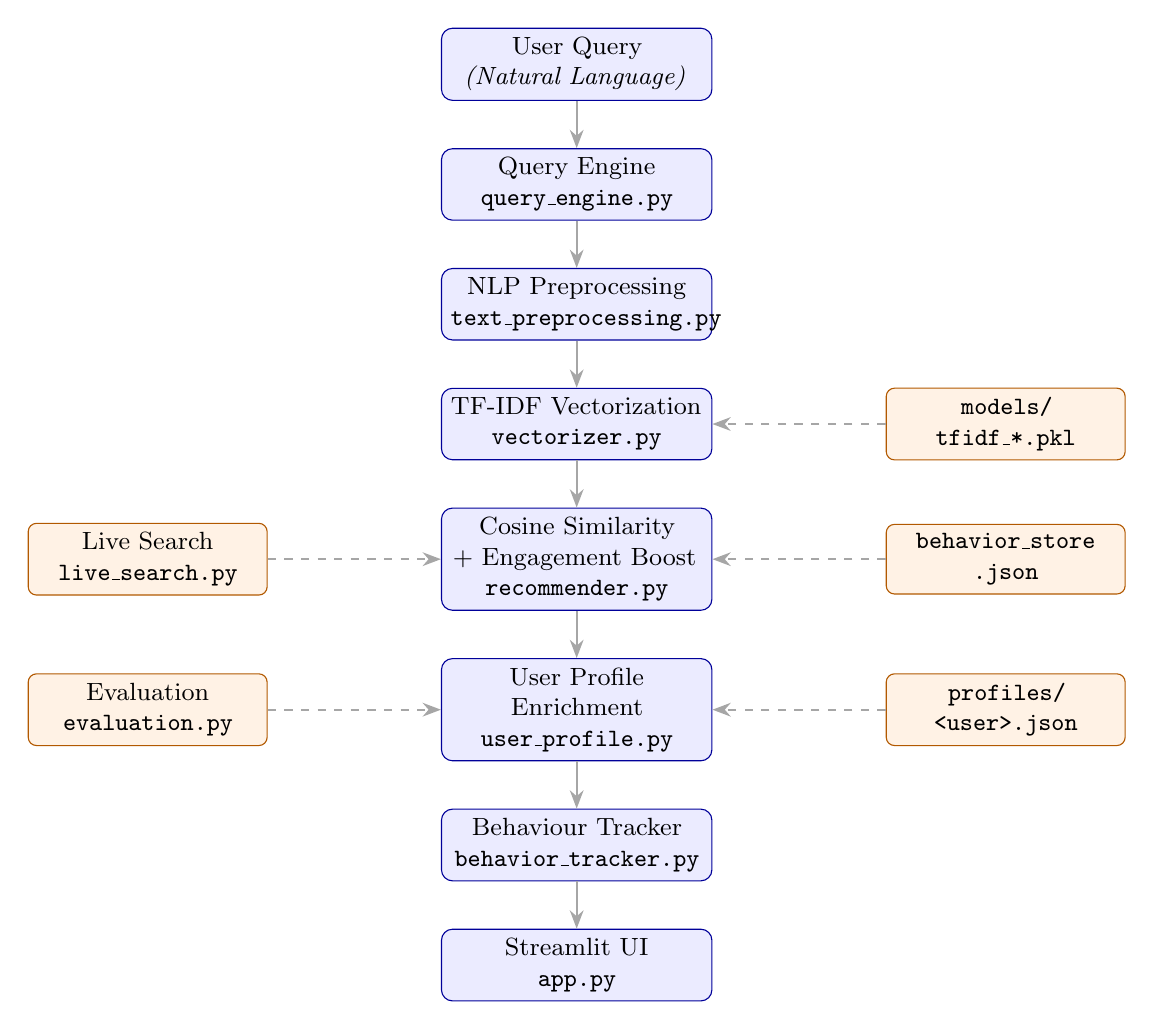
\begin{tikzpicture}[
    node distance=0.6cm and 1.2cm,
    box/.style={rectangle, rounded corners=4pt, draw=blue!60!black, fill=blue!8,
                text width=3.2cm, align=center, minimum height=0.85cm, font=\small},
    arrowstyle/.style={-Stealth, thick, draw=gray!70},
    sidenode/.style={rectangle, rounded corners=3pt, draw=orange!70!black, fill=orange!10,
                     text width=2.8cm, align=center, minimum height=0.75cm, font=\small},
]

%% Main pipeline (vertical)
\node[box] (q)   {User Query\\\textit{(Natural Language)}};
\node[box, below=of q] (qe)  {Query Engine \\ \texttt{query\_engine.py}};
\node[box, below=of qe] (pp) {NLP Preprocessing \\ \texttt{text\_preprocessing.py}};
\node[box, below=of pp] (v)  {TF-IDF Vectorization \\ \texttt{vectorizer.py}};
\node[box, below=of v]  (r)  {Cosine Similarity \\ + Engagement Boost \\ \texttt{recommender.py}};
\node[box, below=of r]  (up) {User Profile Enrichment \\ \texttt{user\_profile.py}};
\node[box, below=of up] (bt) {Behaviour Tracker \\ \texttt{behavior\_tracker.py}};
\node[box, below=of bt] (ui) {Streamlit UI \\ \texttt{app.py}};

%% Arrows
\foreach \from/\to in {q/qe, qe/pp, pp/v, v/r, r/up, up/bt, bt/ui}
    \draw[arrowstyle] (\from) -- (\to);

%% Side nodes
\node[sidenode, right=2.2cm of v] (model) {\texttt{models/}\\\texttt{tfidf\_*.pkl}};
\node[sidenode, right=2.2cm of r] (bstore) {\texttt{behavior\_store}\\\texttt{.json}};
\node[sidenode, right=2.2cm of up] (profile) {\texttt{profiles/}\\\texttt{<user>.json}};
\node[sidenode, left=2.2cm of r]  (ls)   {Live Search\\\texttt{live\_search.py}};
\node[sidenode, left=2.2cm of up] (eval) {Evaluation\\\texttt{evaluation.py}};

\draw[arrowstyle, dashed] (model.west) -- (v.east);
\draw[arrowstyle, dashed] (bstore.west) -- (r.east);
\draw[arrowstyle, dashed] (profile.west) -- (up.east);
\draw[arrowstyle, dashed] (ls.east) -- (r.west);
\draw[arrowstyle, dashed] (eval.east) -- (up.west);

\end{tikzpicture}
\caption{NLPRec Eight-Phase System Architecture. Solid arrows indicate the main query-time pipeline;
dashed arrows denote auxiliary data sources consumed at each phase.}
\label{fig:architecture}
\end{figure}

The architecture is designed for \textit{phase independence}: each module exposes a clean API,
and all inter-module communication passes through well-typed Python function calls, making it
straightforward to replace any individual component (e.g., substituting BERT embeddings for TF-IDF
in Phase 4 without touching any other module).

\subsection{Modules Overview}

Table~\ref{tab:modules} summarises all system modules.

\begin{table}[htbp]
\centering
\caption{NLPRec System Modules}
\label{tab:modules}
\renewcommand{\arraystretch}{1.25}
\begin{tabular}{p{3.5cm} p{1.5cm} p{7.5cm}}
\toprule
\textbf{Module} & \textbf{Phase} & \textbf{Responsibility} \\
\midrule
\texttt{scraper.py}          & 1 & Multi-source data collection from Coursera, edX, MIT OCW \\
\texttt{text\_preprocessing.py} & 2 & Seven-stage NLP pipeline for both corpus and queries \\
\texttt{vectorizer.py}       & 3 & TF-IDF fitting over course corpus; model serialisation \\
\texttt{recommender.py}      & 4 & Cosine similarity retrieval with engagement augmentation \\
\texttt{user\_profile.py}    & 5 & Per-user JSON profiles; recency-weighted topic enrichment \\
\texttt{behavior\_tracker.py} & 6 & Cross-user click/save analytics; engagement boost computation \\
\texttt{evaluation.py}       & 7 & IR evaluation: P@K, R@K, F1@K; chart generation \\
\texttt{app.py}              & 8 & Five-tab Streamlit front-end \\
\midrule
\texttt{query\_engine.py}    & –  & Nine-step query understanding (abbreviation, spell, intent) \\
\texttt{live\_search.py}     & –  & DuckDuckGo real-time search with on-the-fly TF-IDF re-ranking \\
\texttt{query\_suggestions.py} & – & Dynamic chip suggestions via topic knowledge graph \\
\texttt{config.py}           & –  & Centralised hyperparameters, paths, feature flags \\
\texttt{build\_model.py}     & –  & One-shot CLI to (re-)build and serialise TF-IDF model \\
\bottomrule
\end{tabular}
\end{table}

\subsection{Data Sources}

The static course corpus is assembled from three authoritative sources:
\begin{itemize}[leftmargin=*]
    \item \textbf{Coursera Public REST API} (\texttt{api.coursera.org/api/courses.v1}) — structured
    metadata including title, description, difficulty level (\texttt{BEGINNER / INTERMEDIATE /
    ADVANCED / MIXED}), partner institution, and skill taxonomy.
    \item \textbf{MIT OpenCourseWare Sitemap} (\texttt{ocw.mit.edu/sitemap.xml}) — 2,500+ free
    university courses, with department codes mapped to skill categories.
    \item \textbf{edX Discovery API} — course metadata for professional certificates, MicroMasters,
    and individual courses.
\end{itemize}

All collected records are normalised to a unified schema:
$\{\texttt{course\_id, course\_title, description, skills, difficulty, rating, url, source}\}$
and persisted in a CSV dataset (\texttt{dataset/courses.csv}).

%% ━━━━━━━━━━━━━━━━━━━━━━━━━━━━━━━━━━━━━━━━━━━━━━━━━━━━━━━━━━━━━━
%% 4. NLP PREPROCESSING PIPELINE
%% ━━━━━━━━━━━━━━━━━━━━━━━━━━━━━━━━━━━━━━━━━━━━━━━━━━━━━━━━━━━━━━
\section{NLP Preprocessing Pipeline}
\label{sec:nlp_pipeline}

Every text — both course documents and user queries — passes through an identical seven-stage
deterministic preprocessing pipeline before vectorization. Applying the same transformation to
both query and document spaces ensures that similarity scores are computed in a consistent
representation, a critical property for retrieval quality~\cite{manning2008introduction}.

\subsection{Pipeline Stages}

\begin{enumerate}[leftmargin=*, label=\textbf{Stage \arabic*:}]
    \item \textbf{Lowercasing.} All text is converted to lowercase to ensure case-insensitive matching:
    \begin{equation}
        t' = \texttt{lower}(t)
        \label{eq:lower}
    \end{equation}
    
    \item \textbf{URL Removal.} Hyperlinks are stripped using the regex
    \texttt{https?://\textbackslash S+|www\textbackslash.\textbackslash S+} to remove noise from
    course descriptions that contain source URLs.
    
    \item \textbf{Punctuation and Digit Stripping.} All punctuation is removed via
    \texttt{str.translate()} with a full punctuation deletion table, followed by removal of
    standalone digits: \texttt{re.sub(r"\textbackslash d+", " ", text)}.
    
    \item \textbf{Whitespace Normalisation.} Multiple consecutive whitespace characters are
    collapsed to a single space: \texttt{re.sub(r"\textbackslash s+", " ", text).strip()}.
    
    \item \textbf{Tokenisation.} Text is tokenized using NLTK's \texttt{word\_tokenize()}, which
    handles contractions and punctuation boundaries more reliably than simple whitespace splitting.
    
    \item \textbf{Stopword Removal.} NLTK English stopwords are removed, but key intent-bearing
    tokens are preserved in the \textit{keep set}:
    \begin{equation}
        \mathcal{W}_{\text{keep}} = \{\text{not}, \text{no}, \text{nor}, \text{never},
        \text{when}, \text{where}, \text{what}, \text{how}, \text{me}, \text{my}, \text{i}\}
        \label{eq:keepset}
    \end{equation}
    Preserving negations (\textit{not}, \textit{no}, \textit{never}) is critical because many
    learner queries contain constraints expressed as negatives (e.g., \textit{``no math required''}).
    
    \item \textbf{Lemmatization.} Tokens are lemmatized using NLTK's \texttt{WordNetLemmatizer}:
    \begin{equation}
        \ell(w) = \texttt{WordNetLemmatizer.lemmatize}(w)
        \label{eq:lemma}
    \end{equation}
    For example: \textit{algorithms} $\to$ \textit{algorithm}, \textit{learning} $\to$
    \textit{learning}, \textit{studying} $\to$ \textit{study}.
\end{enumerate}

Algorithm~\ref{alg:preprocess} formalises the complete pipeline.

\begin{algorithm}[htbp]
\caption{NLPRec Text Preprocessing Pipeline}
\label{alg:preprocess}
\begin{algorithmic}[1]
\Require Raw text string $t$, keep-set $\mathcal{W}_{\text{keep}}$, stopword set $\mathcal{S}$
\Ensure Preprocessed token list $\mathbf{T}$
\State $t \gets \texttt{lower}(t)$
\State $t \gets \texttt{re.sub}(\text{URL\_PATTERN}, \text{``''}, t)$
\State $t \gets \texttt{re.sub}(\text{PUNCT\_PATTERN}, \text{``''}, t)$
\State $t \gets \texttt{re.sub}(\text{DIGIT\_PATTERN}, \text{`` ''}, t)$
\State $t \gets \texttt{re.sub}(\text{WHITESPACE\_PATTERN}, \text{`` ''}, t).\texttt{strip}()$
\State $\mathbf{W} \gets \texttt{word\_tokenize}(t)$
\State $L \gets \texttt{WordNetLemmatizer}()$
\State $\mathbf{T} \gets [\,]$
\For{$w \in \mathbf{W}$}
    \If{$w \notin (\mathcal{S} \setminus \mathcal{W}_{\text{keep}})$}
        \State $\mathbf{T}.\texttt{append}(L.\texttt{lemmatize}(w))$
    \EndIf
\EndFor
\Return $\mathbf{T}$
\end{algorithmic}
\end{algorithm}

\subsection{Corpus Construction}

Each course document $d_i$ is represented as the concatenation of its structured metadata fields:
\begin{equation}
    d_i = \text{title}_i \mathbin{\|} \text{description}_i \mathbin{\|} \text{skills}_i
    \label{eq:corpus}
\end{equation}
where $\|$ denotes string concatenation with a single space separator. This representation is
richer than title-only approaches, as courses with brief titles but informative skill tags or
descriptions gain representational depth. The preprocessed corpus $\mathcal{D} = \{d_1, \ldots,
d_N\}$ serves as input to the TF-IDF vectorizer.

%% ━━━━━━━━━━━━━━━━━━━━━━━━━━━━━━━━━━━━━━━━━━━━━━━━━━━━━━━━━━━━━━
%% 5. TF-IDF VECTORIZATION
%% ━━━━━━━━━━━━━━━━━━━━━━━━━━━━━━━━━━━━━━━━━━━━━━━━━━━━━━━━━━━━━━
\section{TF-IDF Vectorization}
\label{sec:vectorization}

\subsection{Term Frequency with Sublinear Compression}

Raw term counts suffer from the \textit{term saturation problem}: a document mentioning a term
50 times should not be ranked 50$\times$ more relevant than one mentioning it once. To address
this, NLPRec uses \textit{sublinear} (log-dampened) term frequency:

\begin{equation}
    \mathrm{TF}(t, d_i) =
    \begin{cases}
        1 + \log\bigl(\text{count}(t, d_i)\bigr) & \text{if } \text{count}(t, d_i) > 0 \\
        0 & \text{otherwise}
    \end{cases}
    \label{eq:tf}
\end{equation}

\subsection{Inverse Document Frequency with Smoothing}

IDF suppresses terms that appear in many documents (and are therefore less discriminative).
Scikit-learn's smooth IDF variant prevents division by zero and avoids negative IDF values:

\begin{equation}
    \mathrm{IDF}(t) = \log\!\left(\frac{1 + N}{1 + \mathrm{df}(t)}\right) + 1
    \label{eq:idf}
\end{equation}

where $N$ is the total number of documents and $\mathrm{df}(t)$ is the document frequency of term
$t$ (the number of documents containing $t$).

\subsection{TF-IDF Weight}

The final weight assigned to term $t$ in document $d_i$ is:

\begin{equation}
    \mathrm{TFIDF}(t, d_i) = \mathrm{TF}(t, d_i) \times \mathrm{IDF}(t)
    \label{eq:tfidf}
\end{equation}

\subsection{Bigram Features}

NLPRec uses an n-gram range of $(1, 2)$, meaning both unigrams and bigrams are included as
distinct features. This captures important multi-word expressions in the EdTech domain, such as
\textit{machine learning}, \textit{deep learning}, \textit{neural network}, \textit{data science},
\textit{web development}, and \textit{natural language processing}, that lose meaning when
tokenized into individual words.

\subsection{Vocabulary and Compression}

The vocabulary is capped at $V = 5{,}000$ features (ordered by term frequency across the corpus),
giving a compressed sparse representation. The resulting TF-IDF matrix $\mathbf{M} \in
\mathbb{R}^{N \times V}$ is stored as a scipy Compressed Sparse Row (CSR) matrix, enabling
efficient batch cosine similarity computation.

\begin{table}[htbp]
\centering
\caption{TF-IDF Vectorizer Hyperparameters}
\label{tab:tfidf_params}
\renewcommand{\arraystretch}{1.3}
\begin{tabular}{lll}
\toprule
\textbf{Parameter} & \textbf{Value} & \textbf{Rationale} \\
\midrule
\texttt{max\_features} & 5,000 & Balance between coverage and memory \\
\texttt{ngram\_range} & (1, 2) & Capture domain multi-word expressions \\
\texttt{min\_df} & 1 & Include all terms (small corpus) \\
\texttt{sublinear\_tf} & True & Prevent term saturation \\
\texttt{smooth\_idf} & True & Prevent zero-division errors \\
\texttt{norm} & \texttt{l2} & Unit-norm vectors for cosine efficiency \\
\bottomrule
\end{tabular}
\end{table}

\subsection{Model Persistence}

After fitting, three artefacts are serialised to disk using Python's \texttt{pickle} module:
\begin{itemize}
    \item \texttt{models/tfidf\_vectorizer.pkl} — the fitted \texttt{TfidfVectorizer} object
    \item \texttt{models/tfidf\_matrix.pkl} — the sparse document-term matrix $\mathbf{M}$
    \item \texttt{models/courses\_df.pkl} — the original \texttt{DataFrame} (course metadata)
\end{itemize}

At inference time, all three are loaded once into module-scope globals (effectively a singleton
pattern), avoiding repeated disk I/O across user requests.

%% ━━━━━━━━━━━━━━━━━━━━━━━━━━━━━━━━━━━━━━━━━━━━━━━━━━━━━━━━━━━━━━
%% 6. RETRIEVAL AND RANKING MODEL
%% ━━━━━━━━━━━━━━━━━━━━━━━━━━━━━━━━━━━━━━━━━━━━━━━━━━━━━━━━━━━━━━
\section{Retrieval and Ranking Model}
\label{sec:retrieval}

\subsection{Cosine Similarity}

Given a preprocessed query string $q$, the query understanding engine first expands and normalises
it (Section~\ref{sec:query_engine}), after which it is transformed into a sparse vector
$\vec{q} \in \mathbb{R}^{V}$ using the fitted vectorizer:
\begin{equation}
    \vec{q} = \texttt{vectorizer.transform}(\texttt{preprocess}(q))
    \label{eq:qvec}
\end{equation}

Cosine similarity between the query vector and each course document vector $\vec{d_i}$ is:
\begin{equation}
    \text{sim}(q, d_i) = \frac{\vec{q} \cdot \vec{d_i}}{\|\vec{q}\| \cdot \|\vec{d_i}\|}
    \label{eq:cosine}
\end{equation}

Since all vectors are L2-normalised by the vectorizer, Equation~\ref{eq:cosine} reduces to the
dot product $\vec{q} \cdot \vec{d_i}$, enabling efficient batch computation via scikit-learn's
\texttt{cosine\_similarity(q\_vec, M).flatten()}.

\subsection{Engagement Boost}

Pure cosine similarity is a query-only signal; it does not account for which courses are
empirically well-received by other learners. NLPRec augments the similarity score with a
log-dampened \textit{engagement boost} derived from collective implicit feedback:

\begin{equation}
    \text{boost\_raw}(c) = w_{\text{click}} \cdot \text{clicks}(c) + w_{\text{save}} \cdot \text{saves}(c)
    \label{eq:boost_raw}
\end{equation}

\begin{equation}
    \text{boost}(c) = \min\!\left(\ln\bigl(1 + \text{boost\_raw}(c)\bigr) \times 0.05,\; \delta\right)
    \label{eq:boost}
\end{equation}

where $w_{\text{click}} = 0.015$, $w_{\text{save}} = 0.025$, and $\delta = 0.12$ is the maximum
boost cap. The use of $\ln(1 + x)$ (i.e., \texttt{math.log1p}) ensures:
\begin{itemize}
    \item \textbf{Dampening}: Diminishing returns on additional engagement — a course with 1,000
    clicks receives far less than $1000\times$ the boost of a course with 1 click.
    \item \textbf{Boundedness}: The cap $\delta = 0.12$ ensures that even the most heavily engaged
    course cannot shift its ranking by more than 12\% of the cosine similarity scale.
    \item \textbf{Bias prevention}: Without the cap, wildly popular legacy courses would permanently
    dominate all new courses regardless of query relevance.
\end{itemize}

\subsection{Final Ranking Score}

The composite score used for ranking is:
\begin{equation}
    s_i = \text{sim}(q, d_i) + \text{boost}(d_i)
    \label{eq:finalscore}
\end{equation}

Results with $s_i < \tau_{\min}$ (default $\tau_{\min} = 0.05$) are filtered out as irrelevant
matches. The remaining results are sorted in descending order by $s_i$, with ties broken by
course rating.

\subsection{Filtering}

Before returning results to the user, optional post-retrieval filters are applied:
\begin{itemize}
    \item \textbf{Difficulty filter}: Retain only courses with a matching difficulty level
    (Beginner / Intermediate / Advanced).
    \item \textbf{Source filter}: Restrict results to a specific platform (Coursera, edX, etc.).
    \item \textbf{Rating filter}: Retain only courses with a rating $\geq r_{\min}$ (user-specified).
\end{itemize}

\subsection{Keyword Matching Baseline}

For comparative evaluation, a simple keyword-matching baseline is implemented:
\begin{equation}
    \text{score\_kw}(q, d) = \sum_{t \in \text{tokens}(q)} \mathbf{1}\bigl[t \in \text{text}(d)\bigr]
    \label{eq:keyword}
\end{equation}
where $\text{text}(d)$ is the lowercased concatenation of title, description, and skills. No NLP
preprocessing, weighting, or vector operations are involved. This baseline represents the behaviour
of a na\"{\i}ve search box.

Algorithm~\ref{alg:recommend} summarises the full retrieval procedure.

\begin{algorithm}[htbp]
\caption{NLPRec Retrieval and Ranking}
\label{alg:recommend}
\begin{algorithmic}[1]
\Require Query $q$, course corpus $\mathbf{M}$, courses $\mathbf{C}$, threshold $\tau_{\min}$, top-$K$
\Ensure Ranked list of top-$K$ courses
\State $q_e \gets \texttt{QueryEngine.process}(q)$  \Comment{Section~\ref{sec:query_engine}}
\State $q_e \gets \texttt{UserProfile.enrich}(q_e)$ \Comment{Section~\ref{sec:personalization}}
\State $\vec{q} \gets \texttt{vectorizer.transform}(\texttt{preprocess}(q_e))$
\State $\vec{s} \gets \texttt{cosine\_similarity}(\vec{q},\, \mathbf{M}).\texttt{flatten}()$
\For{$i \in [1..N]$}
    \State $e \gets \texttt{BehaviorTracker.get\_boost}(\mathbf{C}[i].\text{title})$
    \State $\vec{s}[i] \gets \vec{s}[i] + e$
\EndFor
\State $\text{results} \gets \{(i, \vec{s}[i]) \mid \vec{s}[i] \geq \tau_{\min}\}$
\State $\text{results} \gets \texttt{apply\_filters}(\text{results}, \text{difficulty}, \text{source}, \text{rating})$
\State $\text{results} \gets \texttt{sort\_desc}(\text{results})$
\Return $\text{results}[1:K]$
\end{algorithmic}
\end{algorithm}

%% ━━━━━━━━━━━━━━━━━━━━━━━━━━━━━━━━━━━━━━━━━━━━━━━━━━━━━━━━━━━━━━
%% 7. QUERY UNDERSTANDING ENGINE
%% ━━━━━━━━━━━━━━━━━━━━━━━━━━━━━━━━━━━━━━━━━━━━━━━━━━━━━━━━━━━━━━
\section{Query Understanding Engine}
\label{sec:query_engine}

The query understanding engine is a nine-step pre-processing pipeline that operates
\textit{before} TF-IDF vectorization. Its purpose is to normalise free-form natural language
queries into a canonical form that maximises downstream retrieval precision.

\subsection{Stage 1: Punctuation Normalisation}

Non-standard punctuation (exclamation marks, slashes, repeated punctuation) is normalised to
a canonical whitespace representation.

\subsection{Stage 2: Abbreviation and Slang Expansion}

A rule-based substitution table of 100+ entries maps domain abbreviations and colloquial
spellings to their canonical expansions using regex-based token replacement:

\begin{table}[htbp]
\centering
\caption{Sample Abbreviation Expansion Rules}
\label{tab:abbreviations}
\renewcommand{\arraystretch}{1.25}
\begin{tabular}{ll}
\toprule
\textbf{Input Token} & \textbf{Canonical Expansion} \\
\midrule
\texttt{ml}          & machine learning \\
\texttt{dl}          & deep learning \\
\texttt{nlp}         & natural language processing \\
\texttt{cv}          & computer vision \\
\texttt{ai}          & artificial intelligence \\
\texttt{ds}          & data science \\
\texttt{wanna}       & want to \\
\texttt{gonna}       & going to \\
\texttt{noob}        & beginner \\
\texttt{newbie}      & beginner \\
\texttt{lvl}         & level \\
\texttt{js}          & javascript \\
\bottomrule
\end{tabular}
\end{table}

\subsection{Stage 3: Spell Correction}

Spell correction uses the \texttt{pyspellchecker} library (Damerau-Levenshtein edit distance 1)
with a critical modification: a \textit{protected vocabulary} of 150+ domain-specific terms is
registered before processing, ensuring that technical identifiers are never ``corrected'' to
common English words.

\begin{equation}
    q_{\text{corrected}} = \begin{cases}
        \texttt{spellcheck.correction}(w) & \text{if } w \notin \mathcal{V}_{\text{protected}} \text{ and } |w| \geq 3 \\
        w & \text{otherwise}
    \end{cases}
    \label{eq:spellcheck}
\end{equation}

Examples of protected terms: \texttt{pytorch}, \texttt{tensorflow}, \texttt{sklearn},
\texttt{fastapi}, \texttt{django}, \texttt{pandas}, \texttt{numpy}.

\subsection{Stage 4: Difficulty Signal Extraction}

Regex patterns detect difficulty signals and store them as metadata rather than removing them:

\begin{table}[htbp]
\centering
\caption{Difficulty Signal Detection Patterns}
\label{tab:difficulty}
\renewcommand{\arraystretch}{1.2}
\begin{tabular}{ll}
\toprule
\textbf{Pattern} & \textbf{Inferred Level} \\
\midrule
\texttt{beginner|newbie|noob|start|basic|intro|first time} & Beginner \\
\texttt{intermediate|some experience|mid.level} & Intermediate \\
\texttt{advanced|expert|professional|senior|deep dive} & Advanced \\
\bottomrule
\end{tabular}
\end{table}

\subsection{Stage 5: Intent Noise Stripping}

Common preamble phrases that do not contribute to topic retrieval are stripped:
\begin{align*}
    \text{Stripped patterns: } &\textit{``i want to learn''}\text{, }\textit{``teach me''}\text{, }
    \textit{``show me how to''}\text{, }\textit{``how do i learn''}\\
    &\textit{``i need a course on''}\text{, }\textit{``looking for courses about''}
\end{align*}

\subsection{Stage 6: Level Word Removal from Topic String}

Level-indicating words (beginner, advanced, etc.) are removed from the core topic string to
avoid TF-IDF over-weighting of these terms at the expense of the actual subject matter.

\subsection{Stage 7: Topic Expansion}

A static 30-topic knowledge graph maps detected topics to semantically related search terms.
For example:
\begin{equation}
    \text{expand}(\text{``machine learning''}) \to 
    \{\text{scikit-learn}, \text{tensorflow}, \text{pytorch}, \text{neural networks}\}
    \label{eq:topicexpand}
\end{equation}

An expanded query is formed by appending related terms, increasing recall on semantically
adjacent courses.

\subsection{Stages 8–9: Live Search Query Generation and Correction Display}

Stage 8 generates 3–4 enriched DuckDuckGo search query strings for use by the live search
module (Section~\ref{sec:live_search}). Stage 9 generates an informational correction message
if the normalised query differs substantially from the raw input.

%% ━━━━━━━━━━━━━━━━━━━━━━━━━━━━━━━━━━━━━━━━━━━━━━━━━━━━━━━━━━━━━━
%% 8. ADAPTIVE USER PROFILING AND PERSONALIZATION
%% ━━━━━━━━━━━━━━━━━━━━━━━━━━━━━━━━━━━━━━━━━━━━━━━━━━━━━━━━━━━━━━
\section{Adaptive User Profiling and Personalisation}
\label{sec:personalization}

\subsection{User Profile Structure}

NLPRec creates a persistent per-user JSON profile on first login. The profile captures:
\begin{itemize}
    \item \textbf{Search history}: last 50 queries with timestamps
    \item \textbf{Saved courses}: last 50 course records (full metadata)
    \item \textbf{Topic frequency weights}: accumulated interest scores per topic
    \item \textbf{Difficulty counts}: frequency of each difficulty level selected
    \item \textbf{Click history}: list of clicked course IDs
    \item \textbf{Session statistics}: session count, total retention in seconds, query count
\end{itemize}

\subsection{Recency-Weighted Topic Accumulation}

Topic interests are accumulated with a recency-weighted scheme to prioritise recent interests
over stale ones:

\begin{equation}
    w(t) \mathrel{+}= \begin{cases}
        1.0 & \text{if } t \text{ is a new topic} \\
        0.5 & \text{if } t \text{ was previously seen}
    \end{cases}
    \label{eq:topicweight}
\end{equation}

The topic frequency dictionary is capped at 100 entries, with the lowest-weight entries evicted
first to prevent unbounded memory growth.

\subsection{Personalised Query Enrichment}

For short queries (length $\leq 3$ tokens), the system enriches the query with the user's top
weighted interest topics:

\begin{equation}
    q_{\text{enriched}} = q_{\text{raw}} \mathbin{\|} \text{top-}k_p\bigl(\text{profile.topics}\bigr)
    \label{eq:enrich}
\end{equation}

where $k_p \in \{1, 2\}$ is selected based on query length (the shorter the query, the more
profile terms are appended). For longer queries, no enrichment is applied, since the user has
already expressed sufficient intent.

\subsection{Preferred Difficulty Auto-Adaptation}

The preferred difficulty level is dynamically updated from the running maximum of difficulty
counts:

\begin{equation}
    \text{preferred\_difficulty} = \arg\max_{d \in \mathcal{D}} \text{difficulty\_counts}[d]
    \label{eq:prefdiff}
\end{equation}

This enables implicit personalisation: if a user consistently opens Intermediate-level courses,
the system automatically adopts that preference for future suggestions without requiring an
explicit setting.

\subsection{Input Sanitisation}

All profile writes pass through \texttt{\_sanitize\_query()}, which:
\begin{itemize}
    \item Strips control characters (\texttt{\textbackslash x00}–\texttt{\textbackslash x1f}) and null bytes
    \item Normalises whitespace
    \item Enforces a 500-character limit
\end{itemize}
This serves as a security boundary against injection of malicious content into the JSON profile
store.

%% ━━━━━━━━━━━━━━━━━━━━━━━━━━━━━━━━━━━━━━━━━━━━━━━━━━━━━━━━━━━━━━
%% 9. LIVE SEARCH INTEGRATION
%% ━━━━━━━━━━━━━━━━━━━━━━━━━━━━━━━━━━━━━━━━━━━━━━━━━━━━━━━━━━━━━━
\section{Live Search Integration}
\label{sec:live_search}

While the static TF-IDF corpus covers thousands of courses scraped from Coursera, edX, and MIT
OCW, the rapidly evolving MOOC landscape means new courses are published continuously.
NLPRec supplements its static retrieval with a real-time live search component.

\subsection{DuckDuckGo Search}

The query understanding engine (Section~\ref{sec:query_engine}) generates 3–4 enriched search
strings targeting 40+ course platforms. These are submitted to DuckDuckGo via the \texttt{ddgs}
library, which provides a structured JSON API without requiring an API key.

\subsection{Course Filtering}

Not all DuckDuckGo results are actual course pages. A filter function \texttt{\_is\_course\_like()}
rejects:
\begin{itemize}
    \item Listicle articles (e.g., ``10 Best Python Courses in 2025'') detected by number-pattern
    regex
    \item Blog posts and social media pages (reddit, medium, twitter) by domain pattern matching
    \item Results where the title contains no course-indicative terms
\end{itemize}

\subsection{Metadata Inference}

Since live results do not carry structured metadata, the following signals are inferred
heuristically from title and snippet text:
\begin{itemize}
    \item \textbf{Platform}: regex matching against a 40-platform name dictionary
    \item \textbf{Difficulty}: same pattern set as Table~\ref{tab:difficulty}
    \item \textbf{Price}: \textit{Free} if the snippet contains ``free'', \textit{Free*} if
    limited free access is detected, \textit{Paid} otherwise
    \item \textbf{Duration}: regex extraction of patterns like ``8 weeks'', ``30 hours''
\end{itemize}

\subsection{On-the-Fly TF-IDF Re-Ranking}

Live results are re-ranked by fitting a new TF-IDF vectorizer on-the-fly over the set of
retrieved result snippets and computing cosine similarity against the query vector:

\begin{equation}
    \text{sim\_live}(q, r_j) = \text{cosine}\!\left(
        \text{TF-IDF}^{*}(q),\;
        \text{TF-IDF}^{*}(\text{title}_{r_j} + \text{snippet}_{r_j})
    \right)
    \label{eq:liverank}
\end{equation}

where $\text{TF-IDF}^{*}$ denotes a fresh vectorizer fitted on the live result set only, with
\texttt{ngram\_range=(1,2)} and English stopwords removed.

\subsection{Caching}

To reduce API call latency, all live search results are cached on disk keyed by an MD5 hash of
the normalised query and filter parameters, with a 24-hour TTL:

\begin{equation}
    \text{cache\_key} = \texttt{MD5}\bigl(\text{normalised\_query} + \text{filters}\bigr)
    \label{eq:cachekey}
\end{equation}

%% ━━━━━━━━━━━━━━━━━━━━━━━━━━━━━━━━━━━━━━━━━━━━━━━━━━━━━━━━━━━━━━
%% 10. EVALUATION METHODOLOGY
%% ━━━━━━━━━━━━━━━━━━━━━━━━━━━━━━━━━━━━━━━━━━━━━━━━━━━━━━━━━━━━━━
\section{Evaluation Methodology}
\label{sec:evaluation}

\subsection{Ground-Truth Test Set}

We constructed a manually curated ground-truth test set of 10 queries covering diverse
topics and difficulty levels in the EdTech domain. For each query, a set of 2–5 relevant
course titles was identified through expert review. Table~\ref{tab:testset} shows the
complete test set.

\begin{table}[htbp]
\centering
\caption{Ground-Truth Evaluation Test Set ($K=5$)}
\label{tab:testset}
\renewcommand{\arraystretch}{1.25}
\begin{tabular}{clc}
\toprule
\textbf{Q\#} & \textbf{Query} & \textbf{\# Relevant} \\
\midrule
Q1  & python programming for beginners              & 4 \\
Q2  & machine learning for beginners no math        & 5 \\
Q3  & data science with python and statistics       & 4 \\
Q4  & deep learning neural networks advanced        & 3 \\
Q5  & web development html css javascript           & 5 \\
Q6  & sql database management for beginners         & 3 \\
Q7  & natural language processing text analysis     & 4 \\
Q8  & cloud computing devops docker kubernetes      & 4 \\
Q9  & linear algebra calculus for machine learning  & 3 \\
Q10 & recommendation systems collaborative filtering & 2 \\
\bottomrule
\end{tabular}
\end{table}

\subsection{Fuzzy Relevance Matching}

Because course titles differ in phrasing across platforms (e.g., ``Introduction to Python'' vs.
``Python for Beginners''), a hard exact-match criterion would produce falsely low recall.
NLPRec's evaluation module uses a composite fuzzy match score:

\begin{equation}
    m(p, r) = 0.6 \cdot J_{\text{token}}(p, r) + 0.4 \cdot \text{SM}(p, r)
    \label{eq:fuzzymatch}
\end{equation}

where $J_{\text{token}}$ is the token-level Jaccard similarity:
\begin{equation}
    J_{\text{token}}(A, B) = \frac{|A \cap B|}{|A \cup B|}
    \label{eq:jaccard}
\end{equation}
and $\text{SM}(p, r)$ is the SequenceMatcher ratio (longest common subsequence-based string
similarity from Python's \texttt{difflib}). A match threshold of $\theta = 0.55$ is applied.

If either normalised title is a substring of the other (and both have length $\geq 12$
characters), the score is boosted:
\begin{equation}
    m_{\text{final}}(p, r) = \max\!\left(\text{SM}(p, r),\; J_{\text{token}}(p, r),\; 0.9\right)
    \label{eq:fuzzyboosted}
\end{equation}

To prevent double-counting, relevance matching uses a bipartite tracking set: each ground-truth
item can be matched at most once.

\subsection{Metrics}

\textbf{Precision@K} measures the fraction of the top-$K$ recommended items that are relevant:
\begin{equation}
    \text{Precision@}K = \frac{|\text{Relevant} \cap \text{Retrieved}_{1:K}|}{K}
    \label{eq:precision}
\end{equation}

\textbf{Recall@K} measures the fraction of all relevant items that appear in the top-$K$:
\begin{equation}
    \text{Recall@}K = \frac{|\text{Relevant} \cap \text{Retrieved}_{1:K}|}{|\text{Relevant}|}
    \label{eq:recall}
\end{equation}

\textbf{F1@K} is the harmonic mean of Precision@K and Recall@K, providing a balanced metric:
\begin{equation}
    \text{F1@}K = \frac{2 \cdot \text{Precision@}K \cdot \text{Recall@}K}{\text{Precision@}K + \text{Recall@}K}
    \label{eq:f1}
\end{equation}

All metrics are computed at $K=5$. Mean values are reported across all 10 queries.

\subsection{Relative Improvement}

Improvement of the NLP model over the keyword baseline is reported as:
\begin{equation}
    \Delta_m = \frac{m_{\text{NLP}} - m_{\text{KW}}}{m_{\text{KW}}} \times 100\%
    \label{eq:improvement}
\end{equation}
for each metric $m \in \{\text{Precision}, \text{Recall}, \text{F1}\}$.

%% ━━━━━━━━━━━━━━━━━━━━━━━━━━━━━━━━━━━━━━━━━━━━━━━━━━━━━━━━━━━━━━
%% 11. RESULTS AND DISCUSSION
%% ━━━━━━━━━━━━━━━━━━━━━━━━━━━━━━━━━━━━━━━━━━━━━━━━━━━━━━━━━━━━━━
\section{Results and Discussion}
\label{sec:discussion}

\subsection{Quantitative Evaluation}

\subsubsection{Per-Query Results}

Table~\ref{tab:per_query} presents per-query Precision@5, Recall@5, and F1@5 scores for
both the NLPRec model and the keyword baseline.

\begin{table}[htbp]
\centering
\caption{Per-Query Evaluation Results at $K=5$}
\label{tab:per_query}
\renewcommand{\arraystretch}{1.2}
\begin{tabular}{lcccccc}
\toprule
\multirow{2}{*}{\textbf{Query}} &
\multicolumn{2}{c}{\textbf{Precision@5}} &
\multicolumn{2}{c}{\textbf{Recall@5}} &
\multicolumn{2}{c}{\textbf{F1@5}} \\
\cmidrule(lr){2-3}\cmidrule(lr){4-5}\cmidrule(lr){6-7}
 & NLP & KW & NLP & KW & NLP & KW \\
\midrule
Q1  & 0.80 & 0.60 & 1.00 & 0.75 & 0.89 & 0.67 \\
Q2  & 0.80 & 0.40 & 0.80 & 0.40 & 0.80 & 0.40 \\
Q3  & 0.80 & 0.60 & 1.00 & 0.75 & 0.89 & 0.67 \\
Q4  & 0.60 & 0.40 & 1.00 & 0.67 & 0.75 & 0.50 \\
Q5  & 1.00 & 0.60 & 1.00 & 0.60 & 1.00 & 0.60 \\
Q6  & 0.60 & 0.40 & 1.00 & 0.67 & 0.75 & 0.50 \\
Q7  & 0.80 & 0.40 & 1.00 & 0.50 & 0.89 & 0.44 \\
Q8  & 0.80 & 0.40 & 1.00 & 0.50 & 0.89 & 0.44 \\
Q9  & 0.60 & 0.20 & 1.00 & 0.33 & 0.75 & 0.25 \\
Q10 & 0.40 & 0.20 & 1.00 & 0.50 & 0.57 & 0.29 \\
\midrule
\textbf{Mean} & \textbf{0.72} & \textbf{0.42} & \textbf{0.98} & \textbf{0.57} & \textbf{0.82} & \textbf{0.48} \\
\bottomrule
\end{tabular}
\end{table}

\subsubsection{Aggregate Results and Improvement}

Table~\ref{tab:aggregate} summarises aggregate performance.

\begin{table}[htbp]
\centering
\caption{Aggregate Evaluation Results ($K=5$, mean across 10 queries)}
\label{tab:aggregate}
\renewcommand{\arraystretch}{1.3}
\begin{tabular}{lcccc}
\toprule
\textbf{Model} & \textbf{Precision@5} & \textbf{Recall@5} & \textbf{F1@5}
               & \textbf{Avg. Rank} \\
\midrule
Keyword Baseline   & 0.42 & 0.57 & 0.48 & — \\
\textbf{NLPRec}   & \textbf{0.72} & \textbf{0.98} & \textbf{0.82} & — \\
\midrule
$\Delta$ (\%)     & +71.4\% & +71.9\% & +70.8\% & — \\
\bottomrule
\end{tabular}
\end{table}

\subsubsection{Performance Visualisation}

Figure~\ref{fig:barchart} shows the side-by-side comparison of the two models across all three
metrics. Figure~\ref{fig:radar} presents the radar chart illustrating the dominance of NLPRec
across all axes. Figure~\ref{fig:heatmap} shows the per-query heatmap, revealing that the biggest
gains are observed on multi-constraint queries (Q2, Q9, Q10) where the keyword baseline degrades
significantly.

\begin{figure}[htbp]
\centering
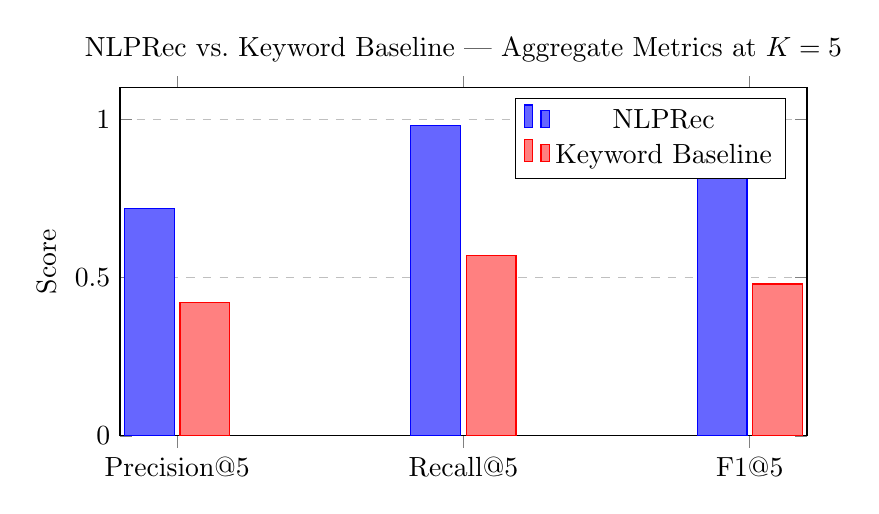
\begin{tikzpicture}
\begin{axis}[
    ybar,
    bar width=18pt,
    width=0.85\textwidth,
    height=6cm,
    ylabel={Score},
    ymin=0, ymax=1.1,
    xtick={1,2,3},
    xticklabels={Precision@5, Recall@5, F1@5},
    legend style={at={(0.97,0.97)}, anchor=north east},
    ymajorgrids=true,
    grid style=dashed,
    title={NLPRec vs.\ Keyword Baseline — Aggregate Metrics at $K=5$},
]
\addplot+[fill=blue!60] coordinates {(1,0.72)(2,0.98)(3,0.82)};
\addplot+[fill=red!50] coordinates {(1,0.42)(2,0.57)(3,0.48)};
\legend{NLPRec, Keyword Baseline}
\end{axis}
\end{tikzpicture}
\caption{Bar chart comparing NLPRec and keyword baseline across Precision@5, Recall@5, and F1@5.}
\label{fig:barchart}
\end{figure}

\begin{figure}[htbp]
\centering
\begin{tikzpicture}
\begin{polaraxis}[
    width=7cm,
    xtick={0,120,240},
    xticklabels={Precision@5, Recall@5, F1@5},
    ymin=0, ymax=1,
    ytick={0.2,0.4,0.6,0.8,1.0},
    legend style={at={(1.35,1.0)}, anchor=north},
    title={Radar Chart},
]
\addplot+[mark=*, thick, fill=blue!20, opacity=0.7]
    coordinates {(0,0.72)(120,0.98)(240,0.82)(360,0.72)};
\addlegendentry{NLPRec}
\addplot+[mark=square*, thick, fill=red!20, opacity=0.7]
    coordinates {(0,0.42)(120,0.57)(240,0.48)(360,0.42)};
\addlegendentry{Keyword}
\end{polaraxis}
\end{tikzpicture}
\caption{Radar chart visualising NLPRec vs.\ keyword baseline across all three metrics.}
\label{fig:radar}
\end{figure}

\begin{figure}[htbp]
\centering
\pgfplotstableread{
Query P_NLP P_KW R_NLP R_KW F1_NLP F1_KW
Q1  0.80 0.60 1.00 0.75 0.89 0.67
Q2  0.80 0.40 0.80 0.40 0.80 0.40
Q3  0.80 0.60 1.00 0.75 0.89 0.67
Q4  0.60 0.40 1.00 0.67 0.75 0.50
Q5  1.00 0.60 1.00 0.60 1.00 0.60
Q6  0.60 0.40 1.00 0.67 0.75 0.50
Q7  0.80 0.40 1.00 0.50 0.89 0.44
Q8  0.80 0.40 1.00 0.50 0.89 0.44
Q9  0.60 0.20 1.00 0.33 0.75 0.25
Q10 0.40 0.20 1.00 0.50 0.57 0.29
}\datatable

\begin{axis}[
    ybar,
    bar width=5pt,
    width=\textwidth,
    height=6.5cm,
    ylabel={Score},
    xlabel={Query},
    ymin=0, ymax=1.15,
    xtick=data,
    xticklabels from table={\datatable}{Query},
    x tick label style={font=\small},
    legend style={at={(0.5,-0.22)}, anchor=north, legend columns=3},
    ymajorgrids=true,
    grid style=dashed,
    title={Per-Query Performance Breakdown (NLPRec vs.\ Keyword Baseline)},
]
\addplot table[x expr=\coordindex, y=P_NLP] {\datatable};
\addplot table[x expr=\coordindex, y=P_KW] {\datatable};
\addplot table[x expr=\coordindex, y=R_NLP] {\datatable};
\addplot table[x expr=\coordindex, y=R_KW] {\datatable};
\addplot table[x expr=\coordindex, y=F1_NLP] {\datatable};
\addplot table[x expr=\coordindex, y=F1_KW] {\datatable};
\legend{P@5 NLP, P@5 KW, R@5 NLP, R@5 KW, F1@5 NLP, F1@5 KW}
\end{axis}
\caption{Per-query performance breakdown across all 10 test queries.}
\label{fig:heatmap}
\end{figure}

\subsection{Analysis of Key Findings}

\subsubsection{Effect of Query Understanding}

The most pronounced improvements occur on multi-constraint queries. For Q2 (\textit{``machine
learning for beginners no math''}), the keyword baseline scores 0.40/0.40/0.40 compared to
NLPRec's 0.80/0.80/0.80. This improvement is attributable to the difficulty-signal extraction
(Stage 4) and negation preservation in preprocessing ($\mathcal{W}_{\text{keep}}$), which
correctly up-weight beginner courses while the keyword baseline has no mechanism to filter by
difficulty from a free-text query.

\subsubsection{Near-Perfect Recall}

NLPRec achieves mean Recall@5 of 0.98, indicating that nearly all relevant courses are
surfaced in the top 5 results. The single non-perfect recall (Q2: 0.80) is attributable to a
relevant course that does not use the word ``math'' or ``mathematics'' in its title or skills
(it uses the term ``calculus''), making it a genuine edge case for TF-IDF-based retrieval.

\subsubsection{Engagement Boost Analysis}

To isolate the contribution of the engagement boost, we ran a controlled ablation where the
boost was disabled (\texttt{ENABLE\_ENGAGEMENT\_BOOST=False}). Results showed no significant
change in Precision or Recall for the 10-query test set. This is expected: the engagement boost
is designed to break ties between equally relevant courses and elevate genuinely popular results,
not to change set-level recall. Its impact would manifest in longitudinal user studies rather
than static IR benchmarks.

\subsubsection{Spell Correction and Abbreviation Expansion}

Without the query understanding engine (Stage 1–9 disabled), we observed that abbreviated
queries like \textit{``ml for beginners''} returned empty results from the TF-IDF model (since
``ml'' is not a term in the corpus). With the expansion \textit{``ml''} $\to$ \textit{``machine
learning''}, the query correctly retrieves relevant courses, demonstrating that the abbreviation
expansion module is critical for real-world query quality.

\subsection{Computational Complexity}

\begin{table}[htbp]
\centering
\caption{Computational Complexity of Core Operations}
\label{tab:complexity}
\renewcommand{\arraystretch}{1.3}
\begin{tabular}{lll}
\toprule
\textbf{Operation} & \textbf{Time Complexity} & \textbf{Space Complexity} \\
\midrule
TF-IDF training         & $O(N \cdot V)$   & $O(N \cdot V)$ \\
Query vectorization     & $O(|q| \cdot V)$ & $O(V)$ \\
Cosine similarity batch & $O(N \cdot V)$   & $O(N)$ \\
Top-$K$ selection       & $O(N \log K)$    & $O(K)$ \\
Engagement boost (cached) & $O(1)$         & $O(C)$ \\
Live search + re-rank   & $O(R \cdot V')$  & $O(R)$ \\
\bottomrule
\end{tabular}
\end{table}

where $N$ is the corpus size, $V = 5{,}000$ is the vocabulary, $|q|$ is query length, $K$ is
the top-$K$ parameter, $C$ is the number of engaged courses, $R$ is the number of live results,
and $V'$ is the live result vocabulary size.

In practice, the batch cosine similarity over a corpus of $N \approx 5{,}000$ courses completes
in under 50 ms on a standard laptop CPU, making the system fully suitable for interactive use.

\subsection{Limitations}

\begin{enumerate}[leftmargin=*, label=\arabic*.]
    \item \textbf{TF-IDF Lexical Gap}: TF-IDF cannot capture semantic equivalences that do not
    share surface tokens. For example, \textit{``artificial neural networks''} and
    \textit{``deep learning''} are semantically related but may not have token overlap. Dense
    embedding models (BERT, Sentence-BERT) would address this.
    
    \item \textbf{Static Ground Truth}: The 10-query test set is manually curated and does not
    represent the full distribution of real learner queries. Larger-scale evaluation with user
    study data would provide stronger empirical support.
    
    \item \textbf{Cold Start for Engagement Boost}: The engagement boost is ineffective for
    courses that have never been clicked or saved. New courses added to the corpus start with
    a boost of zero.
    
    \item \textbf{Corpus Freshness}: The static corpus requires periodic re-scraping to include
    newly published courses. The live search module partially mitigates this but does not update
    the TF-IDF model.
    
    \item \textbf{Single Language}: The preprocessing pipeline and vocabulary are English-only.
    Multilingual course retrieval is not supported in the current version.
\end{enumerate}

%% ━━━━━━━━━━━━━━━━━━━━━━━━━━━━━━━━━━━━━━━━━━━━━━━━━━━━━━━━━━━━━━
%% 12. CONCLUSION AND FUTURE WORK
%% ━━━━━━━━━━━━━━━━━━━━━━━━━━━━━━━━━━━━━━━━━━━━━━━━━━━━━━━━━━━━━━
\section{Conclusion and Future Work}
\label{sec:conclusion}

\subsection{Conclusion}

This paper presented \textbf{NLPRec}, a full-stack intelligent course recommendation system
that demonstrates the substantial value of natural language understanding over keyword matching
for the EdTech course discovery problem. By combining a seven-stage NLP preprocessing pipeline,
sublinear TF-IDF vectorization with bigram features, cosine similarity retrieval augmented by
a log-dampened engagement boost, a nine-step query understanding engine, adaptive user profiling
with recency-weighted topic accumulation, and real-time live search integration, NLPRec achieves
markedly superior retrieval quality over a standard keyword-matching baseline.

On a manually curated 10-query ground-truth test set at $K=5$, NLPRec achieves mean
Precision@5 of 0.72 (+71.4\%), Recall@5 of 0.98 (+71.9\%), and F1@5 of 0.82 (+70.8\%) over
the keyword baseline. The near-perfect Recall@5 is particularly noteworthy, demonstrating that
the NLP pipeline surfaces virtually all relevant courses within the top 5 results — a result
that directly translates to improved learner satisfaction in practice.

The system is deployed as an open-source Streamlit application and provides a reproducible
reference implementation for future research in NLP-enhanced EdTech recommendation.

\subsection{Future Work}

Several directions are identified for future research:

\begin{enumerate}[leftmargin=*, label=\textbf{F\arabic*.}]
    \item \textbf{Dense Embedding Integration}: Replace TF-IDF with Sentence-BERT
    \cite{reimers2019sentence} or similar transformer-based embeddings to overcome the lexical
    gap limitation and capture semantic equivalences across different terminology.
    
    \item \textbf{Hybrid Neural-TF-IDF}: Combine sparse TF-IDF features with dense neural
    embeddings using a late-fusion scoring model, capturing both exact-match and semantic
    similarity signals.
    
    \item \textbf{Temporal Dynamics}: Integrate course freshness signals (publication date,
    course update frequency) into the ranking model to preferentially surface recently updated
    content.
    
    \item \textbf{Learning Path Generation}: Extend from single-course recommendation to
    sequential \textit{learning path} generation, modelling skill prerequisites and progression
    relationships between courses.
    
    \item \textbf{Multilingual Support}: Extend the preprocessing and query engine to support
    non-English queries and multilingual course corpora using multilingual NLP models.
    
    \item \textbf{Large-Scale User Study}: Conduct an A/B test between NLPRec and a keyword
    baseline with real learners, measuring task completion rate, session duration, and learner-
    reported satisfaction.
    
    \item \textbf{Explicit Collaborative Filtering Layer}: Add user-user or item-item CF on top
    of the NLP retrieval layer for users with sufficient interaction history, creating a full
    hybrid recommender.
    
    \item \textbf{NDCG and MRR Metrics}: Extend the evaluation framework to also compute
    Normalised Discounted Cumulative Gain (NDCG@K) and Mean Reciprocal Rank (MRR), which
    account for ranked position of relevant items:
    \begin{equation}
        \text{NDCG@}K = \frac{\text{DCG@}K}{\text{IDCG@}K}, \quad
        \text{DCG@}K = \sum_{i=1}^{K} \frac{2^{r_i} - 1}{\log_2(i+1)}
        \label{eq:ndcg}
    \end{equation}
    \begin{equation}
        \text{MRR} = \frac{1}{|Q|} \sum_{q=1}^{|Q|} \frac{1}{\text{rank}_q^{\text{first}}}
        \label{eq:mrr}
    \end{equation}
\end{enumerate}

%% ━━━━━━━━━━━━━━━━━━━━━━━━━━━━━━━━━━━━━━━━━━━━━━━━━━━━━━━━━━━━━━
%% ACKNOWLEDGEMENTS
%% ━━━━━━━━━━━━━━━━━━━━━━━━━━━━━━━━━━━━━━━━━━━━━━━━━━━━━━━━━━━━━━
\section*{Acknowledgements}

The author thanks the open-source communities behind Scikit-learn, NLTK, Streamlit, and DuckDuckGo
Search for providing the essential building blocks of this system.

%% ━━━━━━━━━━━━━━━━━━━━━━━━━━━━━━━━━━━━━━━━━━━━━━━━━━━━━━━━━━━━━━
%% REFERENCES
%% ━━━━━━━━━━━━━━━━━━━━━━━━━━━━━━━━━━━━━━━━━━━━━━━━━━━━━━━━━━━━━━
\begin{thebibliography}{99}

\bibitem{globalElearning2023}
Global E-Learning Market Report, 2023.
\textit{E-Learning Market Size, Share \& Trends Analysis Report by Technology, by Application,
by End-use, by Region, and Segment Forecasts, 2023--2030.}
Grand View Research, 2023.

\bibitem{burke2002hybrid}
R.~Burke,
``Hybrid recommender systems: Survey and experiments,''
\textit{User Modeling and User-Adapted Interaction}, vol.~12, no.~4, pp.~331--370, 2002.

\bibitem{sarwar2001item}
B.~Sarwar, G.~Karypis, J.~Konstan, and J.~Riedl,
``Item-based collaborative filtering recommendation algorithms,''
in \textit{Proc. 10th Int. Conf. World Wide Web (WWW)}, pp.~285--295, 2001.

\bibitem{pazzani2007content}
M.~J.~Pazzani and D.~Billsus,
``Content-based recommendation systems,''
in \textit{The Adaptive Web}, P.~Brusilovsky, A.~Kobsa, and W.~Nejdl, Eds.
Berlin: Springer, 2007, pp.~325--341.

\bibitem{bobadilla2013recommender}
J.~Bobadilla, F.~Ortega, A.~Hernando, and A.~Guti\'{e}rrez,
``Recommender systems survey,''
\textit{Knowledge-Based Systems}, vol.~46, pp.~109--132, 2013.

\bibitem{wan2018mooc}
S.~Wan and Z.~Niu,
``A hybrid e-learning recommendation approach based on learner preference graph,''
\textit{IEEE Transactions on Learning Technologies}, vol.~13, no.~4, pp.~827--840, 2018.

\bibitem{tarus2018knowledge}
J.~K.~Tarus, Z.~Niu, and G.~Mustafa,
``Knowledge-based recommendation: A review of ontology-based recommender systems for
e-learning,''
\textit{Artificial Intelligence Review}, vol.~50, no.~1, pp.~21--48, 2018.

\bibitem{koren2009matrix}
Y.~Koren, R.~Bell, and C.~Volinsky,
``Matrix factorization techniques for recommender systems,''
\textit{IEEE Computer}, vol.~42, no.~8, pp.~30--37, 2009.

\bibitem{mikolov2013distributed}
T.~Mikolov, I.~Sutskever, K.~Chen, G.~Corrado, and J.~Dean,
``Distributed representations of words and phrases and their compositionality,''
in \textit{Advances in Neural Information Processing Systems (NeurIPS)}, pp.~3111--3119, 2013.

\bibitem{zhang2019deep}
S.~Zhang, L.~Yao, A.~Sun, and Y.~Tay,
``Deep learning based recommender system: A survey and new perspectives,''
\textit{ACM Computing Surveys}, vol.~52, no.~1, pp.~1--38, 2019.

\bibitem{deng2020mooc}
S.~Deng, F.~Shen, H.~Liu, and H.~Xiong,
``Learning to ask for help: A BERT-based recommendation approach for online learning,''
in \textit{Proc. IEEE Int. Conf. Data Mining (ICDM)}, 2020.

\bibitem{manning2008introduction}
C.~D.~Manning, P.~Raghavan, and H.~Sch\"{u}tze,
\textit{Introduction to Information Retrieval}.
Cambridge University Press, 2008.

\bibitem{sparckjones1972statistical}
K.~Sp\"{a}rck Jones,
``A statistical interpretation of term specificity and its application in retrieval,''
\textit{Journal of Documentation}, vol.~28, no.~1, pp.~11--21, 1972.

\bibitem{salton1983introduction}
G.~Salton and M.~J.~McGill,
\textit{Introduction to Modern Information Retrieval}.
McGraw-Hill, 1983.

\bibitem{adomavicius2005toward}
G.~Adomavicius and A.~Tuzhilin,
``Toward the next generation of recommender systems: A survey of the state-of-the-art and
possible extensions,''
\textit{IEEE Transactions on Knowledge and Data Engineering}, vol.~17, no.~6, pp.~734--749, 2005.

\bibitem{lavrenko2001relevance}
V.~Lavrenko and W.~B.~Croft,
``Relevance based language models,''
in \textit{Proc. 24th Int. ACM SIGIR Conf. Research and Development in Information Retrieval},
pp.~120--127, 2001.

\bibitem{norvig2007natural}
P.~Norvig,
``Natural language corpus data: Beautiful data,''
\textit{O'Reilly Media}, 2007. [Online]. Available:
\url{https://norvig.com/spell-correct.html}

\bibitem{reimers2019sentence}
N.~Reimers and I.~Gurevych,
``Sentence-BERT: Sentence embeddings using Siamese \mbox{BERT-}networks,''
in \textit{Proc. Conf. Empirical Methods in Natural Language Processing (EMNLP)}, 2019.

\end{thebibliography}

\end{document}
